%!TEX program = xelatex

\documentclass[onecolumn,a4paper,10pt]{article}

\usepackage[ boldfont,slantfont]{xeCJK}  %设定支持中文
\usepackage{multicol}

\graphicspath{{figures/}}    %设置放置图片的文件夹

\linespread{1.2}     %设置行间距的命令

\setmainfont{Times New Roman}



%for windows fonts
%\setCJKmainfont[BoldFont={SimHei},ItalicFont={KaiTi}]{SimSun}
%\setsansfont{SimHei}
%
%\setCJKfamilyfont{song}{SimSun}
%\setCJKfamilyfont{kai}{KaiTi}
%\setCJKfamilyfont{hei}{SimHei}
%\setCJKfamilyfont{yao}{FZYaoTi}
%
%\newcommand\song{\CJKfamily{song}}
%\newcommand\kai{\CJKfamily{kai}}
%\newcommand\hei{\CJKfamily{hei}}
%\newcommand\yao{\CJKfamily{yao}}

\setCJKmainfont[BoldFont={STXihei},ItalicFont={STKaiti}]{STSong}
\setsansfont{STXihei}

\setCJKfamilyfont{song}{STSong}
\setCJKfamilyfont{kai}{STKaiti}
\setCJKfamilyfont{hei}{STXihei}
%\setCJKfamilyfont{yao}{FZYaoTi}

\newcommand\song{\CJKfamily{song}}
\newcommand\kai{\CJKfamily{kai}}
\newcommand\hei{\CJKfamily{hei}}
%\newcommand\yao{\CJKfamily{yao}}

\newcommand{\erhao}{\fontsize{22pt}{\baselineskip}\selectfont}
\newcommand{\xiaoerhao}{\fontsize{18pt}{\baselineskip}\selectfont}
\newcommand{\sanhao}{\fontsize{16pt}{\baselineskip}\selectfont}
\newcommand{\xiaosanhao}{\fontsize{15pt}{\baselineskip}\selectfont}
\newcommand{\sihao}{\fontsize{14pt}{\baselineskip}\selectfont}
\newcommand{\xiaosihao}{\fontsize{12pt}{\baselineskip}\selectfont}
\newcommand{\wuhao}{\fontsize{10.5pt}{\baselineskip}\selectfont}
\newcommand{\xiaowuhao}{\fontsize{9pt}{\baselineskip}\selectfont}
\newcommand{\liuhao}{\fontsize{7.5pt}{\baselineskip}\selectfont}

%%%段落首行缩进两个字
\makeatletter
\let\@afterindentfalse\@afterindenttrue
\@afterindenttrue
\makeatother
\setlength{\parindent}{2em}%中文缩进两个汉字位


\newcommand{\tabincell}[2]{\begin{tabular}{@{}#1@{}}#2\end{tabular}}

%%%%%%%%%% 定理类环境的定义 %%%%%%%%%%
%% 必须在导入中文环境之后
\newtheorem{example}{例}             % 整体编号
\newtheorem{algorithm}{算法}
\newtheorem{theorem}{定理}[section]  % 按 section 编号
\newtheorem{definition}{定义}
\newtheorem{axiom}{公理}
\newtheorem{property}{性质}
\newtheorem{proposition}{命题}
\newtheorem{lemma}{引理}
\newtheorem{corollary}{推论}
\newtheorem{remark}{注解}
\newtheorem{condition}{条件}
\newtheorem{conclusion}{结论}
\newtheorem{assumption}{假设}

%%%%%%%%%% 一些重定义 %%%%%%%%%%
%% 必须在导入中文环境之后
\renewcommand{\contentsname}{目录}     % 将Contents改为目录
\renewcommand{\abstractname}{摘\ \ 要} % 将Abstract改为摘要
\renewcommand{\refname}{参考文献}      % 将References改为参考文献
\renewcommand{\indexname}{索引}
\renewcommand{\figurename}{图}
\renewcommand{\tablename}{表}
\renewcommand{\appendixname}{附录}
%\renewcommand{\proofname}{证明}
\renewcommand{\algorithm}{算法}

%%%%%%%%%%%%%%%%%%%%%%%%%%%%%%%%%%%%%%%%%%%%%%%%%%%%%%%%%%%%%%%%
%  packages
%    这部分声明需要用到的包
%%%%%%%%%%%%%%%%%%%%%%%%%%%%%%%%%%%%%%%%%%%%%%%%%%%%%%%%%%%%%%%%
\usepackage{graphicx}    % EPS 图片支持
\usepackage{indentfirst} % 中文段落首行缩进
\usepackage{bm}          % 公式中的粗体字符(用命令\boldsymbol)
\usepackage{graphics}	%让文档支持图片
\usepackage{amsmath}	%ams可以让文档支持数学公式
\usepackage{fancyhdr}
\usepackage{fontspec,xunicode,xltxtra}
\usepackage{hyperref}	%让文档支持超链接
\usepackage{booktabs}	%让文档支持三线表格
\usepackage{amsfonts}
%\usepackage{titlesec}
\usepackage{color}
\usepackage{graphicx,psfrag}
\usepackage{epsfig}
\usepackage{verbatim}
\usepackage{picins}
\usepackage{multirow}
\usepackage{listings}
\usepackage{xcolor}
\usepackage[titletoc]{appendix} %附件支持



%%%%%%%%%%%%%%%%%%%%%%%%%%%%%%%%%%%%%%%%%%%%%%%%%%%%%%%%%%%%%%%%
%  lengths
%    下面的命令重定义页面边距,使其符合中文刊物习惯。
%%%%%%%%%%%%%%%%%%%%%%%%%%%%%%%%%%%%%%%%%%%%%%%%%%%%%%%%%%%%%%%%
\addtolength{\topmargin}{-54pt}
\setlength{\oddsidemargin}{0.63cm}  % 3.17cm - 1 inch
\setlength{\evensidemargin}{\oddsidemargin}
\setlength{\textwidth}{14.66cm}
\setlength{\textheight}{24.00cm}    % 24.62
\begin{document}

\bibliographystyle{plain}
%%%%%%%%%%%%%%%%%%%%%%%%%%%%%%%%%%%%%%%%%%%%%%%%%%%%%%%%%%%%%%%%
%  定义标题格式,包括title,author,affiliation,email等。
%  在任何用到中文的地方,用\begin{CJK} ... \end{CJK}将其括起来。
%%%%%%%%%%%%%%%%%%%%%%%%%%%%%%%%%%%%%%%%%%%%%%%%%%%%%%%%%%%%%%%%
\title{\hei{光传输方案}}
\author{肖波\footnote{xbustc@gmail.com}~~~~~~
\\[8pt]
\xiaowuhao 合肥微尺度物质科学国家实验室,安徽~~合肥~~230026\\[4pt]
}
%\date{\today}  % 这一行用来去掉默认的日期显示
\date{\today}
%%%%%%%%%%%%%%%%%%%%%%%%%%%%%%%%%%%%%%%%%%%%%%%%%%%%%%%%%%%%%%%%
%  自定义命令
%%%%%%%%%%%%%%%%%%%%%%%%%%%%%%%%%%%%%%%%%%%%%%%%%%%%%%%%%%%%%%%%
% 此行使文献引用以上标形式显示
\newcommand{\supercite}[1]{\textsuperscript{\cite{#1}}}
%%%%%%%%%%%%%%%%%%%%%%%%%%%%%%%%%%%%%%%%%%%%%%%%%%%%%%%%%%%%%%%%
%  显示title,并设页码为空(按杂志社要求)
%%%%%%%%%%%%%%%%%%%%%%%%%%%%%%%%%%%%%%%%%%%%%%%%%%%%%%%%%%%%%%%%
\maketitle
\pagestyle{fancy}
\lhead{光传输方案}
\cfoot{}
\rfoot{\thepage}
\thispagestyle{empty}
\vspace{-20pt}







\tableofcontents

\newpage


%%%%%%%%%%%%%%%%%%%%%%%%%%%%%%%%%%%%%%%%%%%%%%%%%%%%%%%%%%%%%%%%
%  中文摘要
%%%%%%%%%%%%%%%%%%%%%%%%%%%%%%%%%%%%%%%%%%%%%%%%%%%%%%%%%%%%%%%%

\begin{center}
\parbox{\textwidth}{
%\rule{2em}{0pt}
\hei{摘要:}\song{由于我们MOT可以打的光路有限,为了打入lattice光和其他相关光路并且实现高分辨成像,我们需要将原子从MOT腔传输到科学腔。}\\[5pt]
\hei{关键词:}\song{光传输;气浮平台;绝热}
\\[5pt]
}
\end{center}



\iffalse
%%%%%%%%%%%%%%%%%%%%%%%%%%%%%%%%%%%%%%%%%%%%%%%%%%%%%%%%%%%%%%%%
%  英文摘要
%%%%%%%%%%%%%%%%%%%%%%%%%%%%%%%%%%%%%%%%%%%%%%%%%%%%%%%%%%%%%%%%
\begin{center}
\sihao{\textbf{A \LaTeX{} Template for Chinese Reports}}\\[7pt]
\normalsize
Weiyong Zhang~~~~~~
\\[7pt]
\xiaowuhao Hefei National Laboratory for Physical Sciences at the Microscale, HeFei, AnHui, 230026\\[10pt]
\end{center}
\begin{center}
\parbox{\textwidth}{
\textbf{Abstract:} This is a \LaTeX{} template used for writting documents in Chinese form.\\[4pt]
\textbf{Keywords:} Key; Key; the Key
}
\end{center}
\fi
\section{实验规划}
我们的系统由3个部分组成:2DMOT,3DMOT和科学腔,原子由2DMOT初步冷却再经过3DMOT收集,再由光传输系统移动到科学腔中。光传输基本的原理是通过光与原子的相互作用,利用聚焦的红失谐光将原子囚禁在焦点处,通过移动焦点就可以移动原子的位置实现光传输的目的。目前实现焦点移动的方法中,比较常见的是利用电动平台移动聚焦的透镜或者是移动一组反射镜,另外一种是Tilman Esslinger组使用焦距可变透镜的方法\cite{TTrans},合理的光学设计可以使得焦距变化过程中束腰大小不变,实现绝热的传输。我们的运输距离为228mm左右,但是我们气浮平台传输距离为200mm,所以我们使用通过移动反射镜的方法移动焦点,这个方法的好处是使原子移动距离是平台移动距离的2倍,同时我们使用了一个由焦距为300mm的透镜组成1:1的放大系统,可以将焦点投影到更远的地方,而且这样我们使我们的平台更远离真空腔,减小电机磁场对原子的影响。

我们实验中将使用的fiber coupler A40出来的平行光直径4.3 mm,经过300mm焦距透镜聚焦,理论上能产生$44\mu m$束腰的高斯光,利用2W的光强能够产生$100 \mu K$的势阱。具体的参数可以见图\ref{opticaltransfer}。

\begin{figure}[htbp]
\centering
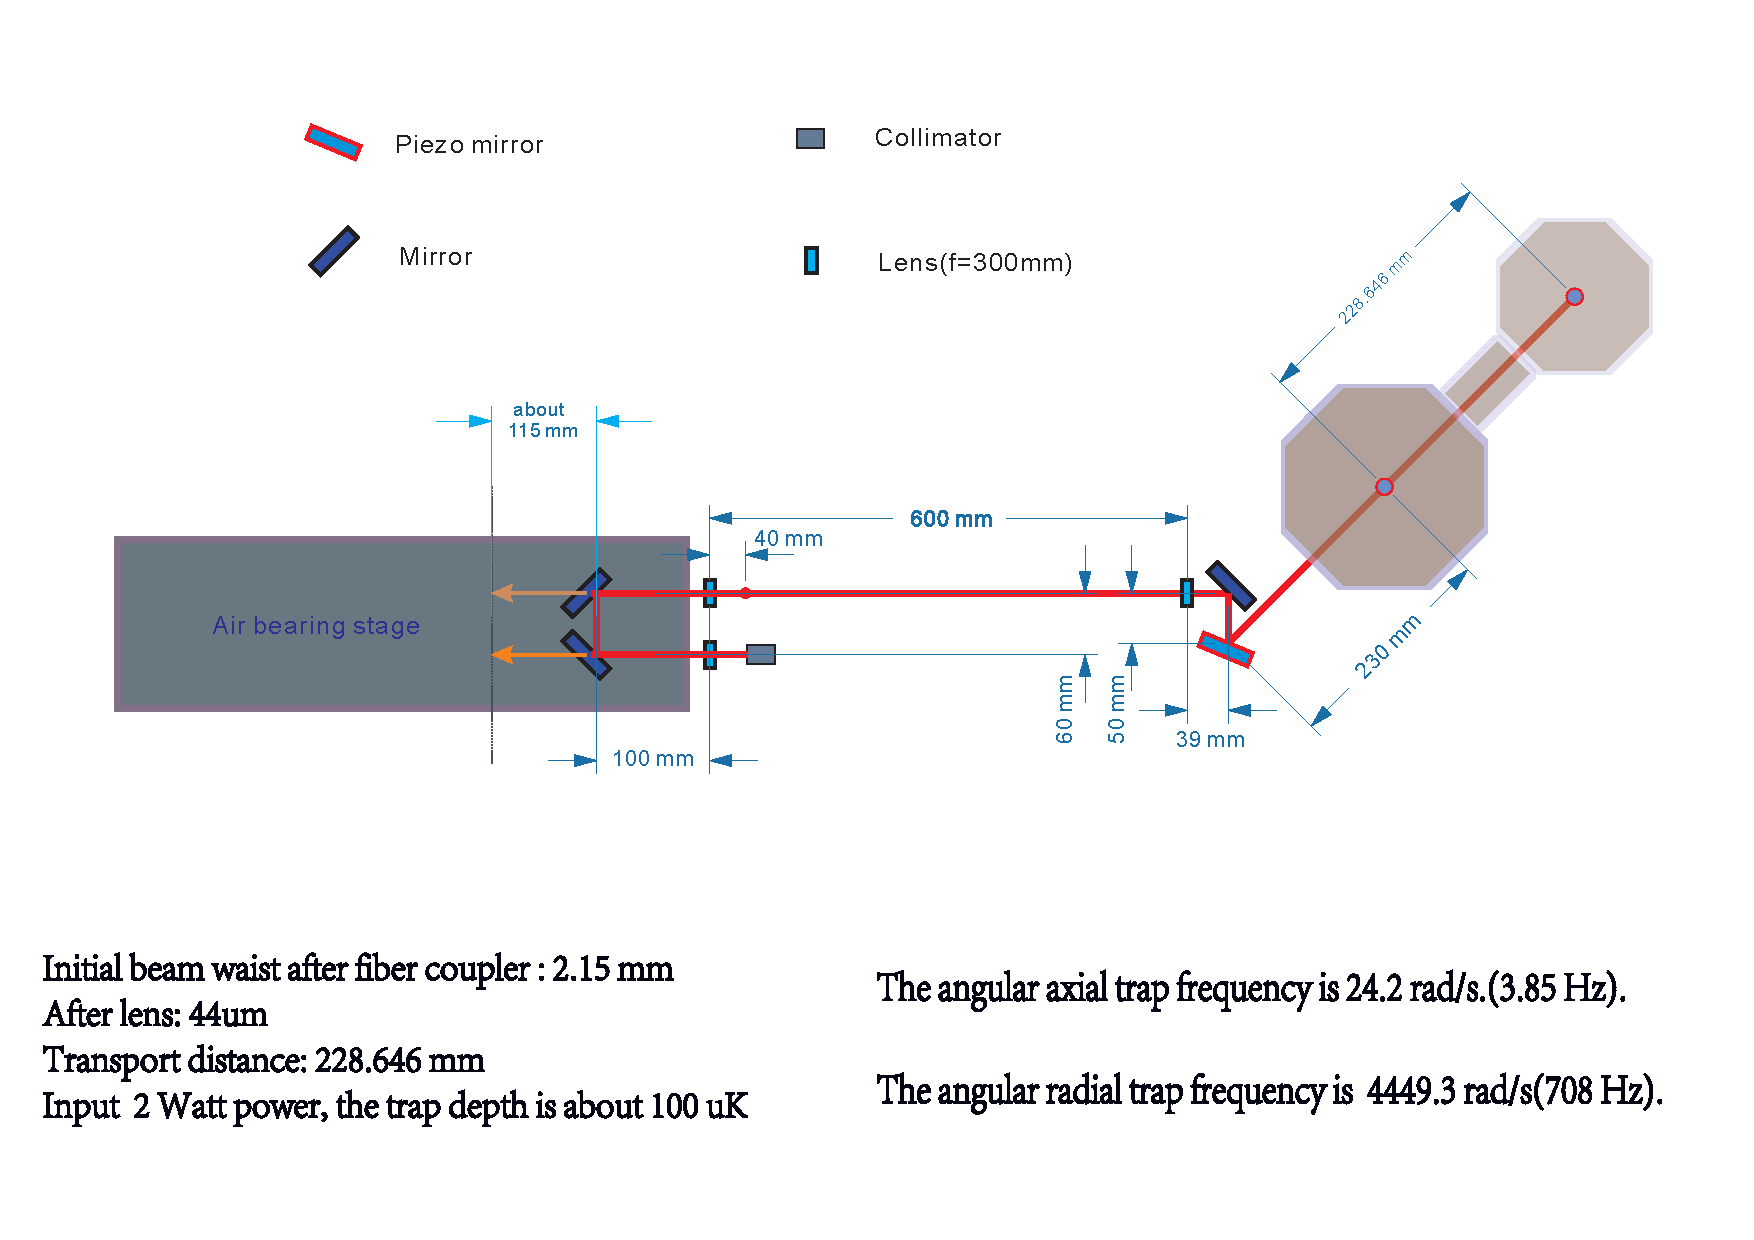
\includegraphics[width=5in]{opticaltransfer.pdf}
\caption{旧光传输方案示意图}
\label{opticaltransfer}
\end{figure}

~\

\textbf{Update-2015.12.18}:

在Markus Geiner组的博士论文\cite{MarkusTrans}中,他们使用的一个2.5倍的放大系统,不但使由第一个移动透镜聚焦平行光得到的束腰可以投影到更远的地方,同时放大后的高斯光束腰移动距离是放大前的$2.5^{2}$倍,见图\ref{Markus}。

\begin{figure}[htbp]
\centering
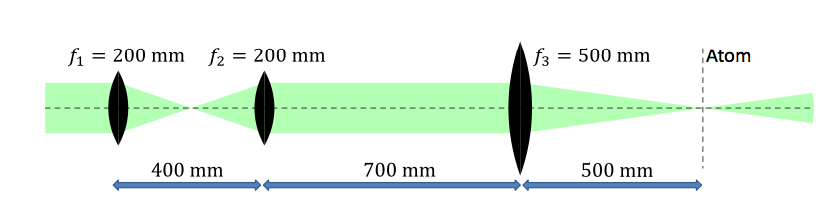
\includegraphics[width=6in]{Markus}
\caption{Markus Greiner组方案}
\label{Markus}
\end{figure}

对于$f_{2}$和$f_{3}$组成的4f成像系统,假设物距为$x$,像距为$x^{'}$,透镜之间的距离为$f_{2}+f_{3}$,我们推导了4f成像系统的像距和物距的关系为

\begin{equation}
	x^{'}=-\frac{xf_{3}^{2}}{f_{2}^{2}}+f_{3}+\frac{f_{3}^{2}}{f_{2}}
\end{equation}
所以,当气浮平台带动第一个透镜移动$\Delta x$,最后的高斯光阱的束腰移动$\Delta x f_{3}^{2}/f_{2}^{2}$,无论束腰是否在前透镜的焦点上,放大系统对于束腰半径的放大倍数始终为$f_{3}/f_{2}$。这个方案的好处是光学元件较少,稳定行更高,之前的方案中需要调节平台上两路光与气浮平台移动方向平行,但这一方案只需一路,但缺点是如果移动透镜前的光不够平行,运输过程中,光阱的束腰会有变化,使得运输过程不够绝热,但理论上束腰变化小于1\%。

最后根据我们的实际情况,我们选用250mm、300mm、400mm为$f_{1}$、$f_{2}$、$f_{3}$的值,移动距离放大16/9,这样我们让气浮平台移动128.25mm,即可使原子移动228mm。同时,为了让光阱的阱足够紧,我们在250mm透镜前面加了-100,50mm的两个透镜将束腰先扩大一倍,这样使得250mm透镜后的光束腰更小,具体参数见图\ref{new}

\begin{figure}[htbp]
\centering
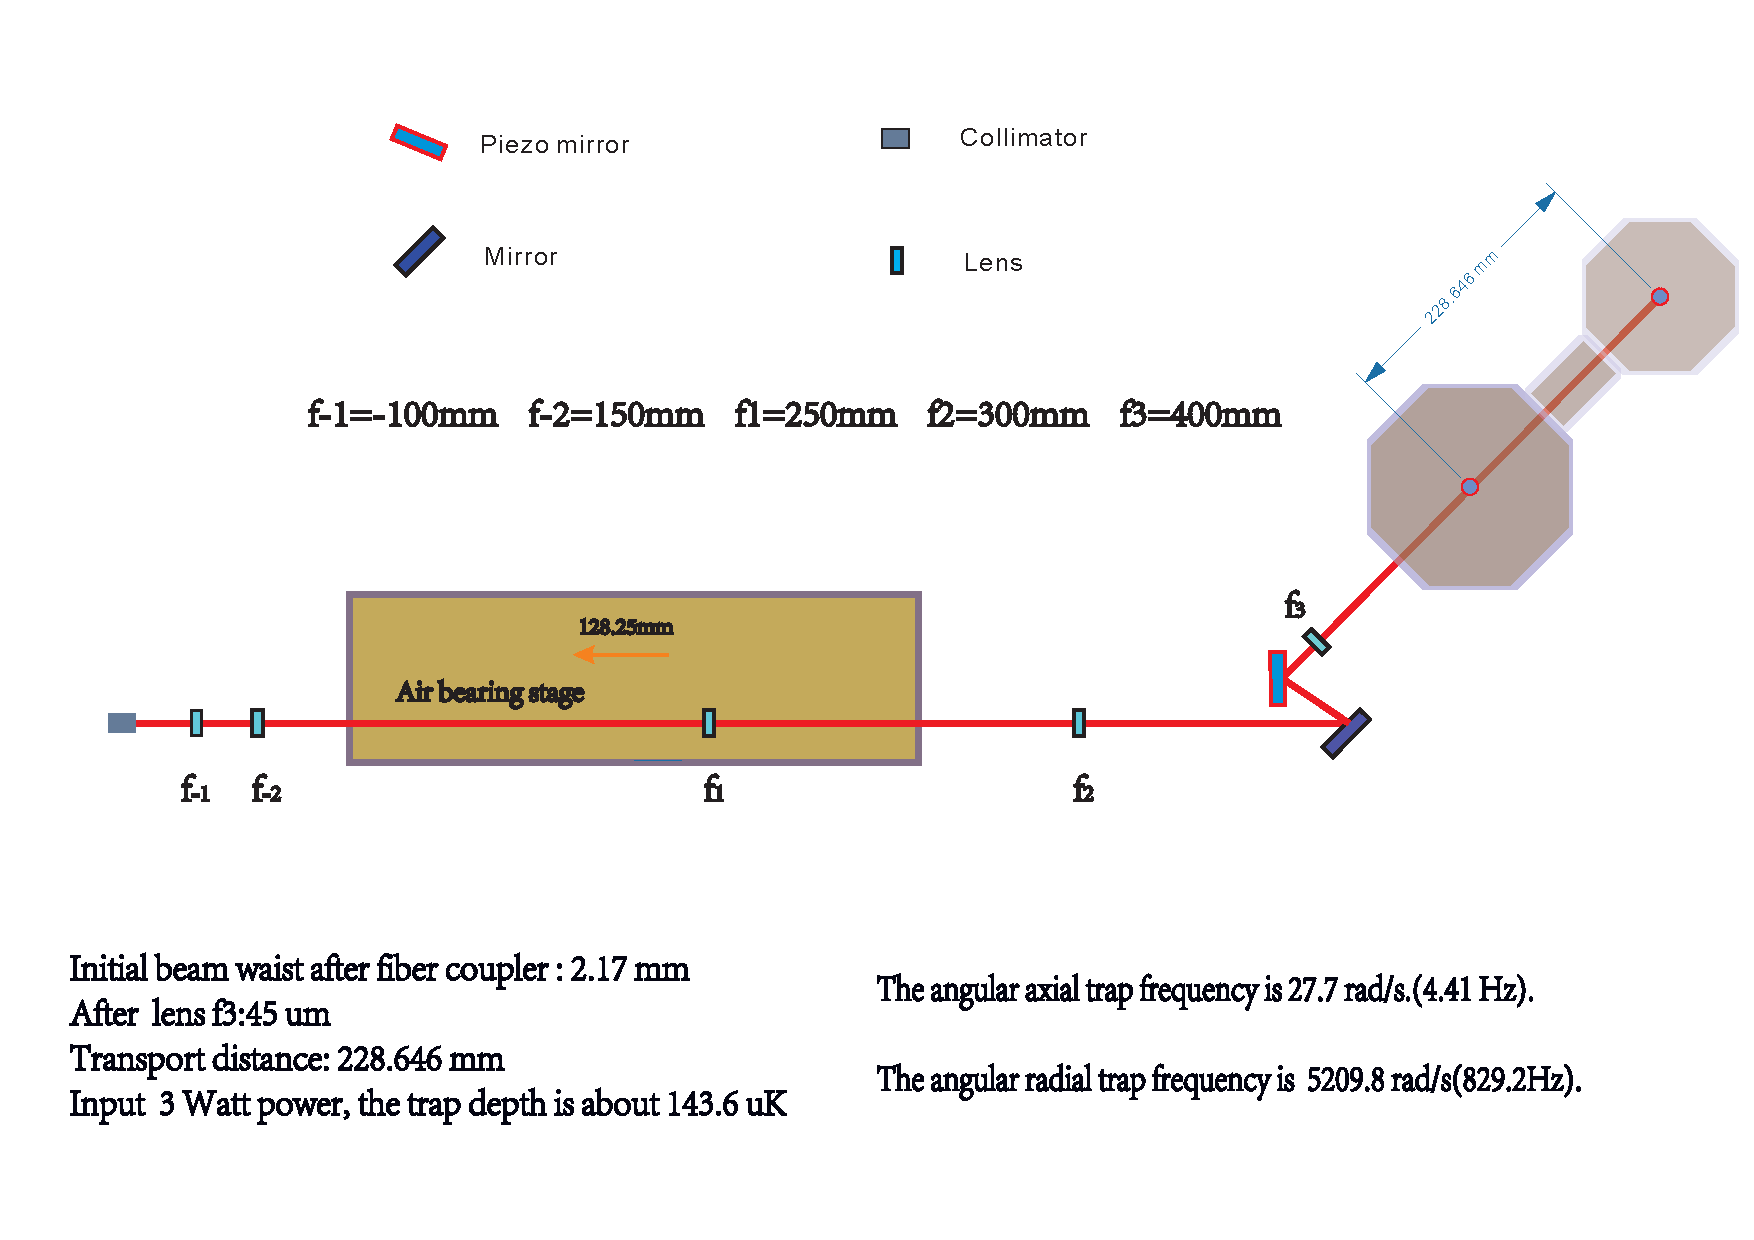
\includegraphics[width=5in]{opticaltransfernew}
\caption{新光传输方案示意图}
\label{new}
\end{figure}

{\color{blue}测量出的最后束腰大小为45um,科学腔最远端观察窗(transfer viewport)距离MOT位置为330mm,在这个位置光的直径为4.96mm;在距MOT位置276mm高分辨观察窗凹下去桶部分边缘,光直径为4.16mm;若采用玻璃腔,玻璃腔离MOT最远的面距离MOT不超过30cm(目前设计为281mm),光在这个位置直径为4.52mm,这些都小于上下玻璃的最小距离5.2mm。}

\section{气浮平台}

在光传输中,光阱的不稳定容易导致原子的加热和损失,光阱的稳定性主要取决于移动的光学元件移动时的稳定性,而这个又由移动平台的性能决定。我们实验中将会使用的是荷兰LAB公司生产的LS200气浮平台,行程为200mm,可移动平台由气体悬浮,所以比一般的直接接触式移动平台具有更高的稳定性。具体的指标参数如表\ref{tab1}所示。
\begin{table}[htbp]
\centering
\label{tab1}
\begin{tabular}{|c|c|}
\hline
Mechaniacal Specifications Travel&200mm\\
\hline
Dimensions of Granite & H240mm|L540mm|W170mm \\
\hline
Dimensions of top plate & 240mm*270mm \\
\hline
Accuracy & ±$0.5 \mu m$\\
\hline
Repeatability & ±$0.1 \mu m$\\
\hline
Straightness &±$0.35 \mu m$\\
\hline
Flatness&±$0.35 \mu m$\\
\hline
Pitch&± 2 arcsec \\
\hline
Roll&± 2 arcsec \\
\hline
Yaw &± 2 arcsec \\
\hline
Load capacity& 300N(V) and 250N(H)\\
\hline

\end{tabular}
\caption{气浮平台性能参数表}
\end{table}

\subsection{供气系统}
由于平台是气浮的,在工作过程中需要对平台内部进行供气,由于精度高,平台对气体压强和洁净度要求很高。我们使用Durr Technik公司生产的Silent Air System产生高压气体,同时使用Festo公司的过滤系统对气体进行过滤,同时加上储气罐和减压阀(festo-529417-MS4-LR-1/4-D6-A5)调节输出气体压强为平台要求的5bar,同时在后面接上SMC公司的干燥管进行干燥,干燥管输出的气体进入平台内部,对平台起到悬浮的作用。

供气系统打开的一般步骤为:
\begin{enumerate}
\item 打开压缩机电源使其开始工作产生高压气体。
\item 用手指抵住第一层过滤单位的底部疏水口,使其内部压缩活塞,将底部密封,当压缩机显示压强到达5bar左右,基本可以松开手指。
\item 等待压缩机输出气压稳定后调节减压阀使其输出压强为5bar。
\item 打开过滤系统后的阀门(1->2)使其与平台内部联通。
\item 当过滤系统所有指示标志为绿色且Driver供气状态显示灯(蓝灯)亮,则说明供气系统工作正常。
\end{enumerate}

当需要关闭整个系统的时候,{\color{red}需等待电机和driver停止工作},关闭阀门(festo-521259-MS4-EM1-1/4-S)和压缩机供电即可。第一次使用以上步骤设置好供气系统,今后每次打开只需要打开阀门和压缩机等待输出气压达到5bar即可。同时,只有空气系统工作正常,才可以为driver供电使平台开始工作。

注:减压阀需要把上面的button往上拔起才可旋转旋钮调节气压。


\subsection{伺服电机}
平台的电机是BOSCH公司生产的MCP020B线性电机,它由driver box提供电流以精确控制它的运动,driver box相当于平台的CPU,计算机向drivebox发出指令以控制平台的运动,driverbox通过USB连接方式和计算机进行通信,计算机通过安装在系统上elmo软件完成这个通信过程。我们可以通过这个软件提供的UI界面定义平台的的速度和位置,也可以类似对CCD和Adwin控制的方法通过写一段程序发送到driverbox的内存里,使driverbox执行程序对平台进行控制,这个也是将来我们主要的工作模式。
\subsection{利用Elmo控制气浮平台}
Elmo软件中,1mm=12800cnts.使用USB线将电脑和drivebox连接起来,用管理员权限打开Elmo软件,在workspace中添加Golddrive设置连接方式为Direct Access USB,同时将与driverbox相连的USB口的编号填入Serial Port USB后,点击connect即可实现计算机和drivebox的连接,连接后软件会自动从driver内存中将所有的设置下载下来,所以基本不用我们设置motor的参数。在Driver Programing中在solution下建立project,一个project下只能有一个程序,将程序填入程序编写窗口,将project link到指定工作的driver上,compile成功后即可点击Build生成img文件载入driverbox中,载入成功后点击Start即可使driverbox执行程序。

通过motion-single Axis界面,我们很方便的设置Unit mode,以及不同mode下的运动参数,这一部分可以用来测试平台的运动,观察平台当前位置和速度的信息以及不同的状态指示灯。Elmo软件还有一个Recorder的功能,可以用来显示一段时间内位置、速度甚至输入输出信号的变化。

Elmo的编程语言基本结构和C语言很像,同时又包含了一些和硬件相关的调用指令。例如BG,IL[N],PV,PTP,JP,HM[N],OB[N]等命令,具体可见command reference guide。

我们需要使用数字信号trigger气浮平台的运动,可以使用IL[1]=7指定Input1输入上升沿为trigger,并且作用为general purpose。程序执行中有判断UI[2]为真的while循环,当为真时则跳出while循环执行运动指令,而UI[2]预设为0,当trigger上升沿输入时,程序中断去执行使UI[2]=1的代码块,这就使得程序能够跳出循环进入运动指令块。



\subsection{绝对位置的标定}

在实际使用过程我们发现,虽然每次使用,软件都会显示一个移动平台的绝对位置,并且有一个参考的零点,但是这个零点在每次平台通电后对应的实际位置都不一样,所以在实际使用过程中,每次通电后,我们都必须对绝对位置进行一个标定,这个标定借助elmo软件中的Homing功能完成。

homing功能使用外部的一个event触发,触发时可以将当前位置的绝对值设定为预设值。一般这个event为一个上升延或者下降沿触发过程,实际过程中可以是home switch、FLS switch或者RLS switch等。home switch软件中只能指定为input5,查看LAB公司给我的输入口对应图,这个input5对应于drive上表明的digit input 2,测试结果也证明了这一点。

参考Tobias Tiecke\cite{Li2DMOT},他们和我们用的是同一家公司的气浮平台,为了矫正绝对位置,他们在平台上使用了一个刀片,在平台边上有一束竖直向下的光束进入光电探测器中,当平台运行到一个位置时,刀片将会开始挡住光,这样光电探测器的输出信号就有一个下降沿,用这个下降沿可以触发homing功能,只要固定光和平台的位置,每次开机用此标定后的绝对位置都能保证一致。

我们采用类似的方法,在平台上立一个刀片,光是从水平方向穿过平台上方进入另一边的光电探测器,当平台到一定位置就会挡住光在光电探测器的输出口产生一个下降沿。我们尝试过使用软件自带的DS402 homing method中第19-22种,采用将input 5设置为home switch的方法去触发homing,一直没有成功。最后我们写了一段代码load到drive中,代码寻找Input5的上升沿,在其上升沿用HM[1]=1指令完成homing的过程。具体的代码如下:


\begin{verbatim}
//this program is used as a homing function. Use digit input 5 as the trigger,
//when the input voltage is high(low), the digit input value is 1(0,respectively),
//When high to low, the rising edge is generated, and trigger HM[1]=1, which sets
//the current position to be 0 or other value you like.

//before using, it's better to choose a good initial position

function main()
HomingZero ()
return
function HomingZero()
UI[2]=0
IL[5]=6 //set Digital input 5 as homing trigger,regard the high level as 0
HM[1]=0
HM[2]=0 // preset homing position value
HM[3]=0
HM[4]=0
HM[5]=0 //set PX= HM[2] when homing
SD=10000

MO=1
until (SO==1)
BG
while(1)
  if    UI[2]
  HM[1]=1 //when trigger comes, set the current position as HM[2]
    break
    end
    JV = 1000
  BG
end
return


#@AUTO_I5
UI[2]=1
return
\end{verbatim}

由于每次homing的时候光强可能不一样,在光电管上输出的电压不一样,这样会导致trigger触发时位置不一样,同时我们发现drive上有模拟输入测量端口,利用这个端口,我们设定当测量到的光强等于初始光强的一半时,进行homing操作,这个可以避免不同天homing光强变化的影响。

%我们采用Agilent的数字万用表34410精度为六位半,最小采样间隔为0.05ms。由于它精度高,我们用它来测试fluxgate的输出,以观测磁场的变化。

\section{光运输的一些参数}
\subsection{基本的运动方程}

原子在光传输过程中得运动可以用以下经典运动方程描述:
\begin{equation}
\ddot{x}_{c}+\omega^{2}_{0}(x_{c}-x_{0}(t))=0
\end{equation}
其中$x_{c}$是原子团质心位置,而$x_{0}(t)$是随时间变化的光阱中心位置。当然原子团的行为也可以用量子力学描述。
任一时刻原子团的能量与初时刻相比变化为
\begin{equation}
	\Delta E(t)=\frac{1}{2} m \dot{x}^{2}_{c}+\frac{1}{2} m \omega^{2}_{0}(x_{c}-x_{0}(t))^{2}
\end{equation}

文献\cite{Trans3}利用量子力学推导出这一能量差可以表示为

\begin{equation}
	\Delta E(t)=\frac{m}{2} |\int_{0}^{t} \ddot{x}_{0}(t^{'})e^{-i\omega_{0}t^{'}}dt^{'}|^{2}
\end{equation}

相对应的原子质心和势阱中心的距离为

\begin{equation}
	\Delta x(t)=\frac{1}{\omega_{0}}\int_{0}^{t}dt^{'} sin[\omega_{0}(t^{'}-t)]\ddot{x}_{c}(t^{'})
\end{equation}

当光传输结束时,如果这个能量不为0,则原子团会围绕势阱中心做简谐运动并由于系统的阻尼而逐渐停止,能量转换为原子团的热运动能量导致原子团的加热。所以我们在设计运动轨迹的时候需要优化曲线来减小这个能量差,减小原子的加热。这个表达式最后等于势阱中心运动速度在阱频率上的傅里叶变化大小。

参考\cite{nonadia},我们采用4-term Blackman-Harris shape作为velocity profile,
\begin{equation}
		\dot{x}_{c}(t)= 0.35875 - 0.48829 cos(2\pi t/T)+0.14128 cos(4\pi t/T)-0.01168cos(6\pi t/T)
\end{equation}

这个shape傅里叶变化下的频谱带宽比较窄,可以有效减小在阱频率上的能量,可以实现robust的光传输,减小光传输结束后原子团围绕势阱中心震荡的振幅,使得过程相对比较绝热。当传输时间$T>8\pi/\omega_{0}$时,振幅基本为0.实际使用的时候需要根据距离在整个表达式前面乘上一个因子。

同时我们也可以使用一些多项式形式的profile进行尝试。例如在设计磁传输运动时在减小加速度变化的要求下计算出的曲线
\begin{equation}
        \dot{x}_{c}(t)= \frac{L}{T}[30(\frac{t}{T})^4-60(\frac{t}{T})^3+30(\frac{t}{T})^2]
\end{equation}

又如Wolfgang Ketterle组\cite{MITTrans}和Markus Greiner组\cite{MarkusTrans},保证整个过程中的jerk(加速度的变化率)不变,在某些拐点处变号。


\subsection{传输时间}
我们的势阱频率设计指标是$2\pi*2.85Hz$和$2\pi*619Hz$,按照Blackman-Harris的要求,传输时间至少要大于1.4s。我们列出不同实验室的传输时间和传输距离作为对比:



\begin{table}[htbp]
\centering
\label{tab2}

\begin{tabular}{|c|c|c|c|c|c|}
\hline
Lab & Time(s)& Distance(cm) &Depth($\mu K$)&Waist($\mu m$)&Remarks\\
\hline
Immanuel Bloch\cite{Singlesite} & 2&13& 100&40&Newport XMS160 stage\\
\hline
Tilman Esslinger\cite{TTrans} & 2-3&28& 147&47&focus-tunable lenses\\
\hline
Wolfgang Ketterle\cite{MITTrans}&2&36&11&24&AeroTech Air-bearing Stage \\
\hline
Tobias Tiecke\cite{Li2DMOT}&3.5&21.5&160&19&LAB-LS Air-bearing Stage \\
\hline
Markus Greiner\cite{MarkusTrans}&3.5&60&Unknown&24&AeroTech Air-bearing Stage \\
\hline

\end{tabular}
\caption{不同实验室传输时间对比}
\end{table}


由于目前我们原子团在光阱中寿命只有6s左右,所以传输时间不能超过这个值,综合考虑,我们将会使用2s左右作为传输时间进行实验。

\section{初步测试结果}
我们于12月底对光传输进行测试,使原子团行进100mm后返回,首先我们使用的是光强为8W的高斯光在molasses中进行装载原子进行光传输,最开始我们使用的是62um的束腰,发现阱频率过低,原子团不能很好的跟谁光阱运动,我们减小束腰到45um,测试效果较好,原子团能够很好的回到初始没有,没有较大的偏差。

我们尝试了正弦、多项式、blackman-barris几种速度曲线,发现正弦曲线原子损失最少,多项式其次,blackman-barris下原子全部丢失。按照统计,使用多项式速度曲线的小组比较多,应该效果最好,但是我们的结果不符这个预期,可能是单向运输多项式可能更好吧,这个需要今后进一步的测试。Blackman-barries理论上是可以最大程度的小于原子到达目的地时的震荡,但是从我们的结果上看,效果并不太好,这个曲线下最大加速度是最大的,可能是阱无法提供这么大的加速度,这个需要今后单向传输时进一步确认。

\textbf{2016-12-18 21:16:04 Update:}

以上测试时在去年进行的,今年的测试发现,在光传输时,光强并不是越强越好,当然这个光强大小主要影响的是前面从磁场蒸发冷却后的原子装载到光阱中的原子的性质,因为我们的光是在磁蒸发开始的时候就在磁阱附近开启以减小Majornona Loss,这个光过强会导致蒸发效果不佳,load到光阱中的原子温度过高导致光传输效率不够,最后我们选定了1W的光强,同时气浮平台如果PID调解不好会在运行时发出响声,经过LAB公司工程师的调解,这一现象解决。







%\section{参考文献}
%%%%%%%%%%%%%%%%%%%%%%%%%%%%%%%%%%%%%%%%%%%%%%%%%%%%%%%%%%%%%%%%
%  参考文献
%%%%%%%%%%%%%%%%%%%%%%%%%%%%%%%%%%%%%%%%%%%%%%%%%%%%%%%%%%%%%%%%
%\section{参考文献}
%%%%%%%%%%%%%%%%%%%%%%%%%%%%%%%%%%%%%%%%%%%%%%%%%%%%%%%%%%%%%%%%
%  参考文献
%%%%%%%%%%%%%%%%%%%%%%%%%%%%%%%%%%%%%%%%%%%%%%%%%%%%%%%%%%%%%%%%
\small

\bibliography{bib/BoXiao}
\end{document}

